\chapter{Keeping Information Secret}
\label{chapter:keepingInformationSecret}

The previous chapter \ref{chapter:representingInformationWithWymbols} was about representing information with symbols. This section is about keeping information secret.
Ciphers haven been used for thousands of years \cite{HistoryOfCryptography}. They are used to keep information secret from people, that are not supposed to have knowledge of it. Not encrypted information is called clear text. Once one encrypted a clear text, it is called a cipher text and only people who know how to decrypt the cipher text can read originally encrypted information.
The exercises in this section are introducing pupils to the concepts of ciphers.

\section{Cipher Texts from Reversed Letters}
\label{section:patterns}

\subsection{Exercises}
The cipher used in these exercises is a simple mix up of letters and both directions are trained: encryption and decryption. In the decryption exercise, the pattern, on which the clear text was encrypted with, is shown. The pupils need to understand the pattern and move the letters in the cipher text accordingly to retrieve the clear text. The encryption exercise is set up analogously. Multiple difficulty levels are possible by changing the amount of moved letters.

\begin{example}
    The cipher text is \code{TNOAM} and the pattern is shown in figure \ref{fig:pattern}. By moving the letter in the cipher text according to the pattern, the clear text can be retrieved: \code{MONAT}.
\end{example}

\begin{figure} 
    \centering
    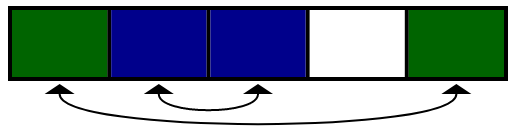
\includegraphics[width=0.4 \columnwidth]{figures/pattern.png}
    \caption{Pattern} 
    \label{fig:pattern} 
\end{figure}

\subsection{Implementation}

Both exercises have a similar implementation. Both need a drawn pattern that indicates the cipher. Fundamentally, the only difference is that for the decryption exercise the given text consists of reversed letters and the solution is compared to the original word, while the encryption exercise gives first the original word as a text and the solution is compared to match the pattern. 
The pattern is created by generating an array of tuples. Each tuple indicates two swapped letters. These two letters are selected randomly and have to be distinct. The exact algorithm used is given in Listing \ref{lst:createPattern}.
Both encryption and decryption exercises have two difficulty levels. They differ by the amount of tuples:

\begin{itemize}
    \item \textbf{easy} - one tuple i.e two swapped letters 
    \item \textbf{medium} - two tuples, i.e in total four swapped letters if the the word has at least four letters, otherwise only two swapped letters 
\end{itemize}

%TC:ignore
\begin{lstlisting}[language=TypeScript,caption={Algorithm to generate an array of distinc tuples of given size},label={lst:createPattern}]
createPattern(text: string[], swapAmount: number): Array<[number, number]> {
  const pattern = new Array<[number, number]>();
  const letters = [...Array(text.length).keys()];
  for (let j = 1; j <= swapAmount && 2 * j <= text.length; j++) {
    const leftIndex = Math.floor(Math.random() * letters.length);
    const left = letters[leftIndex];
    letters.splice(leftIndex, 1);
    const rightIndex = Math.floor(Math.random() * letters.length);
    const right = letters[rightIndex];
    letters.splice(rightIndex, 1);
    pattern.push([Math.min(left, right), Math.max(left, right)]);
  }
  return pattern;
}
\end{lstlisting}
%TC:endignore

The array of tuples needs to be graphically represented. For this purpose the \code{<canvas>} was introduced in HTML5. With the help of scripting language like JavaScript or TypeScript, one can drawn diagrams, edit images and create animations on canvas elements. A canvas element has a height and width and is basically a coordinate system with having the origin in the top left corner at (0, 0). Usually 1 unit corresponds to 1 pixel and all elements are drawn relative to the origin. Some basic operations on a canvas element are drawing rectangles, paths, straight lines, arcs, curves and moving the pen without drawing. Additionally, it can be choosen between filling the drawn structure with a color or only highlighting its border \cite{MDNWebDocs}. These operations already meet the requirements to draw a pattern and requires four steps: 
\TODO{maybe explain canvas in more detail}

\begin{itemize}
  \item \textbf{drawing the grid} - each cell represents a letter of the word
  \item \textbf{colorizing the pairs} - the pairs representing the two letters that need to be swapped are colorize in the same color
  \item \textbf{drawing the arrow heads} - below each cell, that is part of a pair, an arrow head is drawn
  \item \textbf{drawing the arrow lines} - connecting the pairs with lines without the lines overlapping or unnecessarily crossing each other
\end{itemize}

The implementation for these steps is given in listing \ref{lst:createPattern}.

Everything drawn outside of the canvas border is invisible, hence special attenention needs to be given to the first few lines in \ref{lst:createPattern} (L 2-5). When drawing lines, the line width has to be taken into account as well. Therefore, the rectangle is drawn with a distance of half a line width to the actual border of the canvas, so the whole line width is drawn instead of only half of it. 

Drawing the grid includes drawing a rectangle first and  then the lines. To draw the lines, the pen needs to be moved to the start of the line, set down, moved to the end of the line and finally be drawn [\ref{lst:drawGrid}]. 

Drawing a arrow head includes more operations. The pen is first moved the the pointy end of the arrow, set down, moved to the two other corners and back to the pointy end. This time, instead of only highlighting just the border, the whole structure is filled with the black color [\ref{lst:drawArrowHead}].

%TC:ignore
\begin{lstlisting}[language=TypeScript,caption={Implementation to draw the pattern on a canvas element},label={lst:drawPattern}]
drawPattern(cells: number, pairs: [number, number][]) {
  const rectX = this.lineWidth / 2;
  const rectY = this.lineWidth / 2;
  const rectWidth = this.width - this.lineWidth;
  const cellHeight = this.height / 2 - this.lineWidth;
  const cellWidth = rectWidth / cells;

  this.drawGrid(rectX, rectY, rectWidth, cellHeight, cells, cellWidth);

  // sort to have it easier to draw the lines connecting the boxes on the correct height
  pairs.sort(([a, b], [c, d]) => Math.abs(a - b) - Math.abs(c - d));
  const arrowLevelY = this.calculateArrowLevelY(pairs);
  for (let i = 0; i < pairs.length; i++) {
    for (let j = 0; j < 2; j++) {
      const pairIndex = pairs[i][j];

      this.ctx.fillStyle = this.colors[i % this.colors.length];
      this.fillBox(rectX, rectY, cellHeight, cellWidth, pairIndex);

      const centerX = rectX + cellWidth * pairIndex + cellWidth / 2;
      this.ctx.fillStyle = "black";
      this.drawArrowHead(
        centerX,
        rectY + cellHeight + 5,
        Math.min(30, cellWidth),
        10
      );
    }

    this.drawArrowLine(
      cellHeight,
      cellWidth,
      rectY,
      rectX,
      arrowLevelY.get(JSON.stringify(pairs[i])),
      cells,
      pairs[i]
    );
  }
}
\end{lstlisting}
%TC:endignore

%TC:ignore
\begin{lstlisting}[language=TypeScript,caption={},label={lst:drawGrid}]
drawGrid(
  rectX: number,
  rectY: number,
  rectWidth: number,
  cellHeight: number,
  cells: number,
  cellWidth: number
) {
  // draw box
  this.ctx.strokeRect(rectX, rectY, rectWidth, cellHeight);
  // draw walls
  for (let i = 1; i < cells; i++) {
    this.ctx.beginPath();
    this.ctx.moveTo(rectX + cellWidth * i, rectY);
    this.ctx.lineTo(rectX + cellWidth * i, rectY + cellHeight);
    this.ctx.stroke();
  }
}
\end{lstlisting}
%TC:endignore

%TC:ignore
\begin{lstlisting}[language=TypeScript,caption={},label={lst:drawArrowHead}]
drawArrowHead(
  headX: number,
  headY: number,
  headWidth: number,
  headHeight: number
) {
  this.ctx.beginPath();
  this.ctx.moveTo(headX, headY);
  this.ctx.lineTo(headX - headWidth / 2, headY + headHeight);
  this.ctx.lineTo(headX + headWidth / 2, headY + headHeight);
  this.ctx.lineTo(headX, headY);
  this.ctx.fill();
}
\end{lstlisting}
%TC:endignore

\begin{example}
  The pattern in figure \ref{fig:pattern} is generated by calling \code{drawPattern(5, [[0, 4], [1, 2]])} with \code{5} as \code{cells} and \code{[[0, 4], [1, 2]]} as \code{pairs}.
\end{example}

\section{Cipher Texts from New Characters}
\label{section:symbols}

\subsection{Exercises}
Sometimes, only moving symbols in not enough to keep information secret. A better why is to substitute symbols with new symbols. These symbols may be letters, numbers or completly new symbols, that are solely invented for the purpose of encrypting information.
In the following exercises the last approach is followed. Again both direction, encryption and decryption, are trained. But this time, instead of having a pattern, there is a symbol table showing how the letters are encrypted. 

\begin{example}
    The cipher text is shown in figure \ref{fig:cipher_number} and the symbol table in figure \ref{fig:symboltable_numbers}. By using the symbol table one can decrypt the cipher text to \code{52}.
\end{example}

\begin{figure} 
    \centering
    
\includegraphics[width=0.2 \columnwidth]{figures/cipher_number.png}
    \caption{Cipher text of an encrypted number} 
    \label{fig:cipher_number} 
\end{figure}

\begin{figure} 
    \centering
    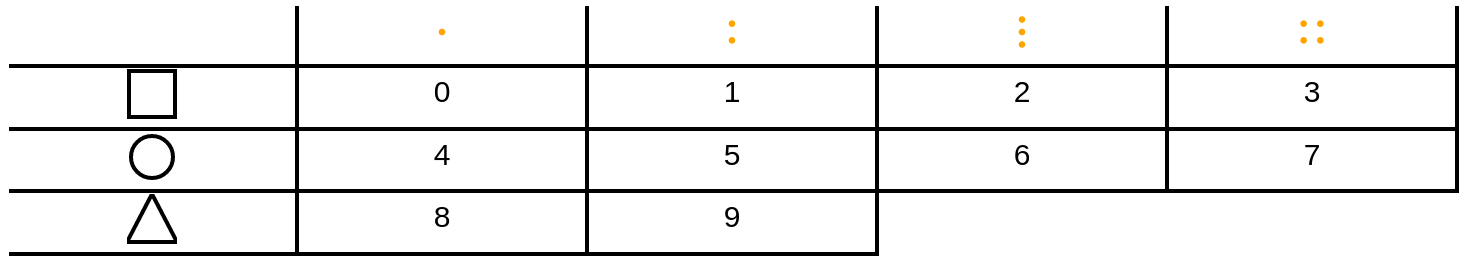
\includegraphics[width=1.0 \columnwidth]{figures/symboltable_numbers.png}
    \caption{Symbol table to encrypt numbers} 
    \label{fig:symboltable_numbers} 
\end{figure}

\subsection{Implementation}

The implementations of the encryption and decryption exercises using symbols are similar to the previous exercises using patterns. The main difference is he use of a symbol table showing what alphanumerical letter is encrypted with what symbol. A symbol is composed of two shapes and the composition configuration is shown in the symbol table. In the decryption exercise a with symbols encrypted text is shown. Pupils have to use the symbol table to translate symbols to its alphanumerical counter part, decrypting the text. In the encryption exercise, it is the other way around. Pupils have to encrypt a text with the help of the symbol table.
The symbol table is implemented in the \code{SymbolTable.vue} component. It accepts a two-dimensional array representing the table content and generates this table with the help of canvas elements. Each cell in the table is a canvas element. Each shape consist of multipe elements e.g the yellow shape in the symbols for numbers consists of multiple points. If there are three or less points, the points are drawn in a vertical line and for four points, they are drawn in grid style. Other shapes are more complex, like the yellow shapes in the symbols for letters consisting of multiple arcs. The implementation for drawing these shapes takes as an argument the amount of arcs that need to be drawn and first draws the straight vertical lines and then the specified amount of arcs. This way this implementation can be used for all three arc shapes [\ref{lst:drawArcs}] used in symbol table [\ref{fig:symboltable_letters}]. 
All other shapes are implemented in a similar way, so there is as less code as possible.

\begin{figure} 
    \centering
    
\includegraphics[width=0.4 \columnwidth]{figures/cipher_text.png}
    \caption{Cipher text of an encrypted text} 
    \label{fig:cipher_text} 
\end{figure}

\begin{figure} 
    \centering
    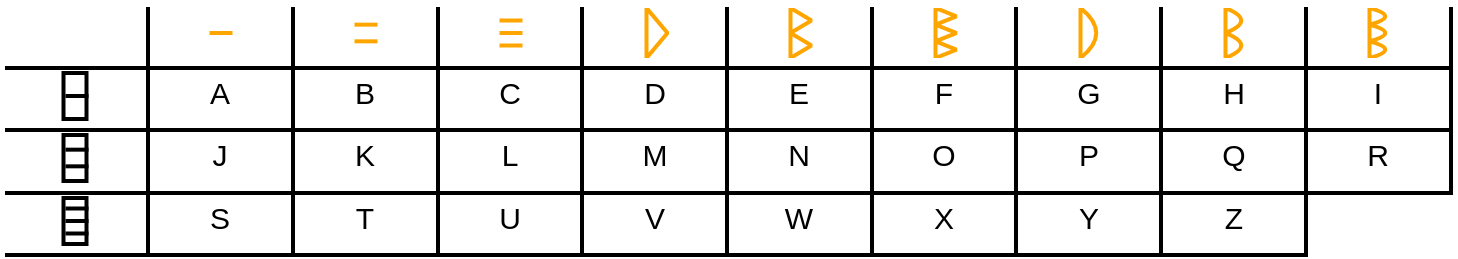
\includegraphics[width=1.0 \columnwidth]{figures/symboltable_letters.png}
    \caption{Symbol table to encrypt and decrypt letters} 
    \label{fig:symboltable_letters} 
\end{figure}

% TC:ignore
\begin{lstlisting}[language=TypeScript,caption={Implementation of drawing a variable amount of arc symbols},label={lst:drawArcs}]
drawArcs(arcs: number) {
  this.ctx.strokeStyle = "#ffa500";
  if (arcs <= 0) {
    return;
  }
  this.ctx.lineJoin = "bevel";
  this.ctx.beginPath();
  this.ctx.moveTo(this.lineWidth / 2, this.height - this.lineWidth / 2);
  this.ctx.lineTo(this.lineWidth / 2, this.lineWidth / 2);
  const diffY = (this.height - this.lineWidth) / (2 * arcs);
  for (let i = 1; i <= arcs; i++) {
    this.ctx.quadraticCurveTo(
      this.width - this.lineWidth / 2,
      (2 * i - 1) * diffY,
      this.lineWidth / 2,
      2 * i * diffY
    );
  }
  this.ctx.stroke();
}
\end{lstlisting}
% TC:endignore
